%---------------------------------- Evaluation Function -------------------------------
\begin{frame}{Evaluate the solution}
    Use LitGPT framework with it's CLI to perform an evaluation of a solution. All models and datasets are taken from HuggingFace Hub.
    \begin{block}{Training}
        \begin{itemize}
            \item Model : Llama-3.2-1B
            \item dataset : Alpaca
            \item 1 epochs of training
            \item Fully Sharded Data Parallelism (FSDP) as distributed strategy
        \end{itemize}
    \end{block}

    \begin{block}{Evaluating}
        Based on lm\_eval library
        \begin{itemize}
            \item validation dataset : Hellaswag
            \item testing dataset : MMLU
        \end{itemize}
    \end{block}

    
\end{frame}

%---------------------------------- BO-GP -------------------------------
\begin{frame}{SMBO : Bayesian-Optimization based on Gaussian-Process (BO-GP)}
    \begin{columns}
        \begin{column}{0.4\textwidth}

            \begin{block}{Principe :}
                \begin{itemize}
                    \item Build a surrogate of the objective function
                    \item Optimize the surrogate to find the most promising point to evaluate
                \end{itemize}
                
            \end{block}
            
        \end{column}        
        \begin{column}{0.5\textwidth}
            \begin{figure}
                \centering
                \usepgfplotslibrary[fillbetween]
\begin{tikzpicture}[domain = 0:5,scale = 0.6]

    \begin{axis}[
        xlabel={$x$},
        ylabel={$y=f(x)$},
        legend pos=outer north east,
        ymin = 2.5,ymax=5, 
        xmin = 0, xmax = 5
    ]
    % plot function
    \addplot [no markers, blue, dashdotted, thick,visible on =<-3>] {sin(\x r)^2+sqrt(\x+8)};
    \addlegendentry[visible on =<-3>]{Function : $f(x)$}

    % Add sampling
    % LHS
    \addplot [blue, only marks, mark = *,visible on =<2-3>] table {assets/tikz_picture/gaussian_process/lhs.dat};
    \addlegendentry[visible on =<2-3>]{Sampled points (LHS)}

    
    \draw[color=teal!50, dashed,visible on =<2>](axis cs:1.25, -5) -- (axis cs:1.25, 27);
    \draw[color=teal!50, dashed,visible on =<2>](axis cs:2.5, -5) -- (axis cs:2.5, 27);
    \draw[color=teal!50, dashed,visible on =<2>](axis cs:3.75, -5) -- (axis cs:3.75, 27);

    % Surrogate
    \addplot [red,visible on =<3-3>] table {assets/tikz_picture/gaussian_process/mean.dat};
    \addlegendentry[visible on =<3-3>]{Surrogate : $\hat{f}(x)$}
    % UCB
    \addplot [violet,dashed,visible on =<3>] table {assets/tikz_picture/gaussian_process/ucb.dat};
    \addlegendentry[visible on =<3>]{Conf. Bnd:$\hat{f}(x) \pm \beta \hat{\sigma}(x)$ }
    % LCB
    \addplot [violet,dashed,visible on =<3>] table {assets/tikz_picture/gaussian_process/lcb.dat};
    \addlegendentry[visible on = <3>]{}

    % Optimize UCB
    \addplot [violet,visible on =<4>] table {assets/tikz_picture/gaussian_process/ucb.dat};
    \addlegendentry[visible on =<4>]{Upper Conf. Bnd. }

    % Local Search 1 : 
        \addplot [violet,visible on =<4>, mark = triangle*,mark size = 3, mark indices = {16,20,25},only marks, mark options = {rotate = 90, color = blue!50}] table {assets/tikz_picture/gaussian_process/ucb.dat}; 
        \addplot [violet,visible on =<4>, mark = triangle*,mark size = 4, mark indices = {27},only marks, mark options = { color = blue}] table {assets/tikz_picture/gaussian_process/ucb.dat};
    % Local Search 2
        \addplot [violet,visible on =<4>, mark = triangle*,mark size = 3, mark indices = {40,35,45},only marks, mark options  = {rotate = 180, color = teal!50}] table {assets/tikz_picture/gaussian_process/ucb.dat};
        \addplot [violet,visible on =<4>, mark = triangle*,mark size = 4, mark indices = {33},only marks, mark options = {color = teal}] table {assets/tikz_picture/gaussian_process/ucb.dat};
    % Local Search 3
        \addplot [violet,visible on =<4>, mark = triangle*,mark size = 3, mark indices = {60,65,70,75},only marks, mark options = {rotate = 90, color = red!50}] table {assets/tikz_picture/gaussian_process/ucb.dat}; 
        \addplot [violet,visible on =<4>, mark = triangle*,mark size = 4, mark indices = {79},only marks, mark options  = {color = red}] table {assets/tikz_picture/gaussian_process/ucb.dat};
    % Best final
    \draw[color=red!50, dashed,visible on =<4>](axis cs:0.79*5, -5) -- (axis cs:0.79*5, 27);



    \end{axis} 

    \onslide<2->\node[font = \small] at (8,2){Etape :};

    \onslide<2>{\node[anchor = west,font = \small] at (8.6,2){Echantillonage};}
    \onslide<3>{\node[anchor = west,font = \small] at (8.6,2){Fit GP};}
    \onslide<4>{\node[anchor = west,font = \small] at (8.6,2){Opt. UCB};}

\end{tikzpicture}
            \end{figure}
        \end{column}
    \end{columns}
    
\end{frame}

%---------------------------------- SOO -------------------------------
\begin{frame}{PBO : Simultaneous Optimistic Optimization(SOO)}
    \begin{columns}
        \begin{column}[b]{0.4\textwidth}
            \textbf{Partition Based Algorithm : Simultaneous Optimistic Optimization (SOO)}

            Perform a K-inary partition of the space, evaluating every center of partition during the expansion of a node.
            
        \end{column}        
        \begin{column}{0.6\textwidth}
            \begin{figure}[h]
                \centering
                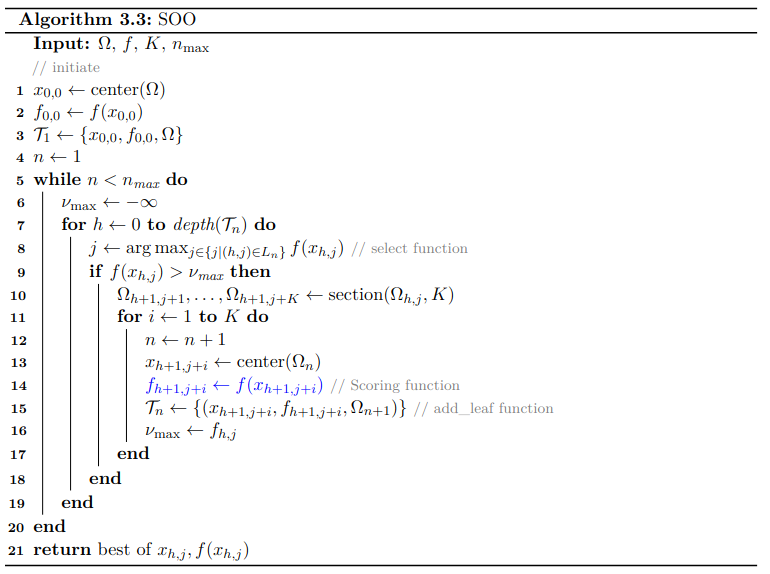
\includegraphics[trim={0 0 7cm 0},clip,height = 6.5cm]{imgs/algo/soo.png}
                \caption{SOO Algorithm}
            \end{figure}
        \end{column}
    \end{columns}
\end{frame}

%---------------------------------- BaMSOO -------------------------------
\begin{frame}{Hybridization : Bayesian Multi-Scale Optimistic Optimization (BaMSOO)}
    \begin{columns}
        \begin{column}{0.5\textwidth}
            \textbf{Hybridation : Bayesian Multi-Scale Optimistic Optimization(BaMSOO)}

            Replace the scoring of SOO with a BO-GP based approximation to determine if it's relevant to evaluate the point.
            \begin{equation}
                \begin{split}
                \mathcal{UCB}(x| \mathcal D_t) = \mu(x|\mathcal D_t) +  B_N * \sigma(x|\mathcal D_t) 
                \\ \text{with } B_N = \sqrt{2 \log (\pi^2 N^2/6 \eta)} , \eta \in (0,1)      
                \end{split}  
                \label{eq:ucb}
            \end{equation}
            
        \end{column}        
        \begin{column}{0.5\textwidth}
            \begin{figure}[h]
                \centering
                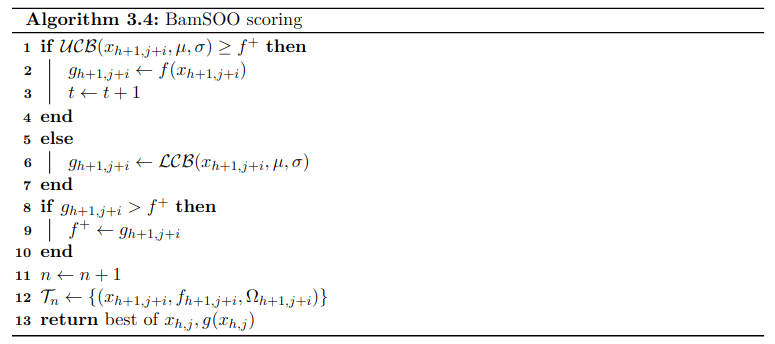
\includegraphics[trim={0 0 12cm 0},clip,height = 5cm]{imgs/algo/bamsoo_score.png}
            \end{figure}
        \end{column}
    \end{columns}
\end{frame}